\documentclass[12pt,a4paper,oneside]{book}

	\makeatletter
	\newcommand\thefontsize[1]{{}}
	\makeatother
	\usepackage[utf8]{inputenc}
	\usepackage{enumitem}
	\usepackage{varwidth}
	\usepackage{graphicx}
	\usepackage{caption}
	
\usepackage[top=2.5cm, bottom=3cm, left=2.5cm, right=2.5cm]{geometry}
\usepackage[utf8]{inputenc}
\usepackage[titletoc,title]{appendix}
\usepackage[linewidth=1pt]{mdframed}
\usepackage{framed}
\usepackage{listings}
\usepackage{smartdiagram}
\usepackage{smartdiagram}
\usepackage{varwidth}
\usepackage{amsmath}
\usesmartdiagramlibrary{additions}
\lstdefinestyle{customc}{
	belowcaptionskip=1\baselineskip,
	breaklines=true,
	frame=L,
	xleftmargin=\parindent,
	language=C,
	showstringspaces=false,
	basicstyle=\footnotesize\ttfamily,
	keywordstyle=\bfseries\color{green!40!black},
	commentstyle=\itshape\color{purple!40!black},
	identifierstyle=\color{blue},
	stringstyle=\color{orange},
}

\lstdefinestyle{customasm}{
	belowcaptionskip=1\baselineskip,
	frame=L,
	xleftmargin=\parindent,
	language=[x86masm]Assembler,
	basicstyle=\footnotesize\ttfamily,
	commentstyle=\itshape\color{purple!40!black},
}

\lstset{escapechar=@,style=customc}

\lstset{
	literate=%
	{à}{{\'a}}1
	{í}{{\'i}}1
	{é}{{\'e}}1
	{è}{{\`e}}1
	{ý}{{\'y}}1
	{ú}{{\'u}}1
	{ó}{{\'o}}1
	{ě}{{\v{e}}}1
	{š}{{\v{s}}}1
	{č}{{\v{c}}}1
	{ř}{{\v{r}}}1
	{ž}{{\v{z}}}1
	{ď}{{\v{d}}}1
	{ť}{{\v{t}}}1
	{ň}{{\v{n}}}1
	{ů}{{\r{u}}}1
	{Á}{{\'A}}1
	{Í}{{\'I}}1
	{É}{{\'E}}1
	{Ý}{{\'Y}}1
	{Ú}{{\'U}}1
	{Ó}{{\'O}}1
	{Ě}{{\v{E}}}1
	{Š}{{\v{S}}}1
	{Č}{{\v{C}}}1
	{Ř}{{\v{R}}}1
	{Ž}{{\v{Z}}}1
	{Ď}{{\v{D}}}1
	{Ť}{{\v{T}}}1
	{Ň}{{\v{N}}}1
	{Ů}{{\r{U}}}1
}

\begin{document}
	\def\reportnumber{}
	\def\reporttitle{Chapitres 1, 2 et 3}
	%----------------------------------------------------------------------------------------
%	TITLE PAGE
%----------------------------------------------------------------------------------------

\begin{titlepage} % Suppresses displaying the page number on the title page and the subsequent page counts as page 1
	\newcommand{\HRule}{\rule{\linewidth}{0.5mm}} % Defines a new command for horizontal lines, change thickness here
	
	\center % Centre everything on the page
	
	%------------------------------------------------
	%	Headings
	%------------------------------------------------
	
	\baselineskip=2\baselineskip 
	\textsc{\LARGE Université des Sciences et de la Technologie Houari Boumediene}%\\[1cm] % Main heading such as the name of your university/college

	%------------------------------------------------
	%	Logo
	%------------------------------------------------
	
	%\vfill\vfill
	\vfill
	
\includegraphics[width=0.3\textwidth]{USTHB_Logo.png}\\[1cm] % Include a department/university logo - this will require the graphicx package
	 
	%----------------------------------------------------------------------------------------
	
	\textsc{\Large Data Mining }\\[0.5cm] % Major heading such as course name
	%\textsc{\large Minor Heading}\\[0.5cm] % Minor heading such as course title
	
	%------------------------------------------------
	%	Title
	%------------------------------------------------
	
	\HRule\\[0.4cm]
	\baselineskip=1.2\baselineskip 
	{\huge\bfseries Résumé du livre "Data Mining
		Concepts and Techniques"\textdegree  \reportnumber \\ \reporttitle}\\[0.4cm] % Title of your document
	
	\HRule\\[1.5cm]
	
	%------------------------------------------------
	%	Author(s)
	%------------------------------------------------
	
	\begin{minipage}{0.4\textwidth}
		\begin{flushleft}
			\large
			\textit{Rédaction:}\\
			MOULAI \textsc{Hassina Safaa}\\ % Your name
			Matricule : 201400007564\\ 
			
			HOUACINE \textsc{Naila Aziza}\\ % Your name
			Matricule : 201400007594\\ 
			
			M2 SII Groupe:3\\
			
		\end{flushleft}
	\end{minipage}
	~
	\begin{minipage}{0.4\textwidth}
		\begin{flushright}
			\large
			\textit{Professeur}\\
			Mme. BABA ALI  % Supervisor's name
		\end{flushright}
	\end{minipage}
	
	%------------------------------------------------
	%	Date
	%------------------------------------------------
	
	\vfill\vfill\vfill % Position the date 3/4 down the remaining page
	
	{\large\today} % Date, change the \today to a set date if you want to be precise
	
	
	\vfill % Push the date up 1/4 of the remaining page
	
\end{titlepage}
	
	
	\sffamily

\setcounter{tocdepth}{1}
\tableofcontents
\newpage

\chapter{Introduction[1]}
% \section{Pourquoi le Data mining }
l'apparition est du  à la richesse du monde actuel en données et l'abondance  de ces derniers  mais paradoxalement pauvre  en information ,  la croissance exponentielle en quantité de données qui sont stockées et collectées sont à l'origine de l'incapacité humaine à gérer ce flux  de données et en extraire des connaissances pertinentes sans une utilisation d'outils adéquates, le besoin en exploration de données grandit et.

\section{Qu'est ce que le Data mining}
Le Data mining ou fouille de données est le processus d'exploration et d'extraction de connaissances ou de motifs à partir d'un volume conséquent de données en utilisant des outils ,
le processus comporte plusieurs étapes qui sont les suivantes :
\subsection{Nettoyage de données}
ceci consiste à éliminer les données bruitées 
\subsection{Integration de données}

\subsection{Sélection de données}
on récupéré les données pertinentes de la base de données pour qu'elles puissent
par la suite être utilisé lors de l'analyse
\subsection{Transformation de données}
La transformation consiste à faire des opérations d'agrégation , normalisation ou bien un résumé à fin de rendre les données sous une formes approprié  pour l'exploration minière .  
\subsection{Data mining}
c'est l'application de méthodes intelligentes pour l'extraction des modèles ou motifs de données 
\subsection{Évaluation des motifs}
c'est une Identification des motifs pertinents représentant le mieux la connaissance

\subsection{Présentation de données}
c'est la visualisation et présentation des connaissances aux utilisateurs.
\section{Les types de données qui peuvent être utilisé pour le data mining }
Ils existent différent types de données sur les quelles le data mining peut opérer , pour cella la seule condition suffisante est que ces données doivent avoir du sens , parmi elles :
\subsection{Les bases de données}
c'est une collection de données interdépendantes  un logiciel  (système de gestion de base de données SGBD) permettant de gérer ,accéder et sécuriser ces données, les données sont sous forme de tables relationnelles  suivant un certain format, chaque table comporte des colonnes qui appelées attribues et les lignes sont les tuples  ou instance ( un objet ).


\subsection{Les entrepôts de données}

un entrepôt de données est un référentiel des informations collectées à partir de sources multiples, stockées sous une base de données unifiée.
ce schéma est résidant généralement sur un site unique, l'entrepôt de données est construit via un processus de nettoyage des données, d’intégration, de transformation, de chargement et de
rafraîchissement des données odiques et généralement modélisé par une structure de données multidimensionnelle, appelée
cube de données
dans lequel chaque
dimension représente un ou plusieurs attributs ,ce cube de données fournit une vue multidimensionnelle des données et permet
le précalcul et l'accès rapide aux données résumées.
\subsection{Base données transactionnelles }
une base de données transactionnelles se compose principalement de transactions mais peut aussi contenir des tables supplémentaires contenant des informations sur les transactions existantes .
\subsection{Autres types de données}
il existe d'autres types de données
sous formes et  structures polyvalentes et assez différentes
sémantiquement. Ces types de données peuvent être vus dans de nombreuses applications: liées au temps
données séquentielles,
les flux de données , données spatiales (cartes, par exemple), données de conception technique , hypertexte et multi-données multimédia (y compris texte, image, vidéo et audio), graphique et données en réseau
et le Web . Ces applications apportent de nouveaux
défis, tel que la gestion des données contenant des structures spéciales et une sémantique spécifique
\section{Quelles sont les motifs qui peuvent être extraites ?}
\subsection{Classe/Concept Description: Caractérisation
	et Discrimination}
Les entrées de données peuvent être associé à des classes ou des concepts , ces classes et concepts sont décrites selon un mécanisme 
de \textbf{caractérisation des données}, en résumant les données de la classe étudiée (souvent appelé le classe cible) en termes généraux, ou \textbf{discrimination des données}, par comparaison de la classe  cible avec une ou plusieurs classes comparatives (souvent appelée la en contraste Des classes),ou une composition des deux techniques. 
le résultat de caractérisation donnent en sortie des statistiques résumé en diagramme à barres
,
courbes , ou bien des règles de généralisations , alors que la discrimination donne en sortie des règles de discriminations.
\subsection{Motifs fréquents , associations et corrélations} 
Les motifs fréquents sont des modèles qui apparaissent de façon assez répétitive dans les données, il existe plusieurs types tel que  les ensembles d'éléments fréquent,des sous-projets ou encore des sous-structures fréquentes séquentiels et structurés  de différentes formes  (graphes,arbre ...),    
\textbf{Association}
les règles d’association sont des règles exprimés  en prédicat permettant de découvrir une relation entre différente variable (attributs) dans une large base de données . \\
\textbf{correlation } est une relation  liant deux ou plusieurs attributs associées dans un large volume de données.
\subsection{Classification et régression pour une analyse prédictive}
La Classification
est le processus de recherche d'un
modèle
(ou fonction) qui décrit et distingue
des classes de données ou des concepts.
ils sont utilisé
pour prédire l'étiquette de classe d'objets pour laquelle l'étiquette de classe est inconnue 

\textbf{  Régression}
régression modélise des fonctions à valeurs continue , c'est une méthode statistique  très utilisée pour prédire les données manquantes ou valeurs indisponibles de données numériques
plutôt que des étiquettes de classe (discrètes).
\subsection{clustering}
Le clustering est le processus de regroupement des objets (des données) selon un degré de similarité entre eux, tel que  on maximise la similarité entre les membres d'un même groupe  tout en minimisant la similarité  entres les membres  de groupes différents (dissimilarité) . ça permet une meilleure organisation de données où chaque groupe présentent une classe ,catégorie ...
\subsection{Outlier (valeurs aberrantes )}
Ce sont des objets non conformes au comportement ou au modèle général des données. Ces objets de données sont valeurs aberrantes. ces objets peuvent être vu comme du bruit ou des exceptions .
\subsection{Ce qui fait qu'un modèle est intéressent}
Il est clair que le data mining peut générer des milliers de modèles et motifs mais l'utilité des modèles restent relatif selon le besoin , à noter que les modèles sont coûteux à produire donc il faudrait s'intéresser qu'aux modèles pertinents, pour qualifier un modèle de tel adjectif il faut :
\begin{itemize}
	\item qu'il soit facile à assimiler et comprendre par ces utilisateurs
	\item qu'il procure une validation de nouvelles données ou d'essai avec un certain degré de certitude
	\item utile et intéressent dans le sens ou il valide ce que l'utilisateur cherche à confirmer ceci donnera naissance à DES CONNAISSANCES
\end{itemize}

.
\section{Quelles genre de technologies sont appliquées et utilisées dans le data mining ?}
\subsection{Statistique}
les statistiques étudient la collection, l'analyse, l'interprétation ou l'explication et la présentation de données.UNE modèle statistique est un ensemble de fonctions mathématiques décrivant le comportement de les objets d'une classe cible en termes de variables aléatoires et leurs distributions . on peut citer la moyenne , la médian , la variance et l'écart type.

\subsection{Machine learning (apprentissage automatique)}
Apprentissage machine étudie comment les ordinateurs peuvent apprendre basé sur des données.
Un domaine de recherche principal concerne les programmes informatiques qui apprennent automatiquement  à reconnaître des modèles complexes et prendre des décisions intelligentes basées sur des données. 
on distingue deux types d'apprentissage supervisé (prédire une classe )et non supervisé (clustering par exemple ) ,Semi-supervisé ,active learning 
\subsection{Système de base de données et entrepôts de données}
La recherche de systèmes de bases de données se concentre sur la création, la maintenance et l'utilisation de bases de données pour les organisations et les utilisateurs .
ces systèmes sont utilisé pour les raisons suivantes :
les modèles de données, les langages de requête, le traitement des requêtes,méthodes d’optimisation, stockage de données et méthodes d’indexation et d’accès qui permet une meilleure exploration de données.

on note aussi  l'entrepôt qui consolide
les données dans un espace multidimensionnel pour former des cubes de données facilitant ainsi leurs explorations .

\subsection{Recherche d'information}
recherche d'information(IR) est la science de la recherche de documents ou d'informations dans les documents.ils peuvent être du texte ou du multimédia et peuvent résider sur le Web .La recherche d'informations suppose que  les données sous recherche sont non structurées et les requêtes sont formées principalement par des mots-clés.

\section{Quelles sont les genres d'applications ciblé par le data mining}
\subsection{Business intelligence}
La technologie de l'intelligence d'entreprise  (BI) fournit des informations historiques, actuelles et
vues prédictives des opérations commerciales. 
ceci en incluant les rapports, l'analyse en ligne
traitement, gestion des performances de l'entreprise, veille concurrentielle, analyse comparative et analyse prédictive de comportement des clients par exemple .
\subsection{Web  Search engine }
Un Moteur de recherche Web est un serveur informatique spécialisé dans la recherche des informations sur le Web , les résultats de la recherche d’une requête utilisateur sont souvent renvoyés sous forme de liste,les types des résultats peuvent consister en des pages Web, des images et d’autres types de fichiers.
\section{Les problèmes qui font face au data mining}
Il y a beaucoup de défis en jeux de la recherche en exploration de données:
\begin{itemize}
	\item  La méthodologie minere
	\item Interaction avec l'utilisateur
	\item  L'efficacité et l'évolutivité, et la gestion de diverses Types de données
\end{itemize}



\chapter{Connaitre vos données[1]}

Dans Data Mining il y a "DATA", Ainsi nous nous devons tout d'abord d'étudier les caractéristiques des attributs et des valeurs de nos données avant de passer au pré-traitement. 
et ce car les données de nos Dataset collectées du monde réel contiennent du bruit, aussi elles proviennent de divers sources donc elles ne sont pas homogènes en plus de l'énorme volume qu'elles constituent.
Cette étape consiste principalement en:\\
\textbf{ }
Trouver le type de valeur que peut prendre chaque attribut et si elles sont discrètes ou continues, Avoir une idée d'à quoi ressemble nos données et de leur distribution, Chercher quelle méthode de visualisation nous donnerai un meilleur aperçu, Mesurer le degré de similarité entre certaines données et Calculer les statistiques de base concernant chaque attribut


\section{Type des attributs d'un Dataset}
Un Dataset est un ensemble d'Objets dit données, échantillons ou tuples.
 Ces données sont généralement décrites par des attributs.\\
 Ainsi dans ce qui suit nous allons plus nous intéresser aux types d'attributs existants.
 
\subsection{Définition d'un attribut}
Un attribut est un domaine de données, représentant une caractéristique de cette dernière. 
Un ensemble d'attributs aussi dit vecteur d'attribut est utilisé pour décrire un objet.\\
Il y a plusieurs manières de définir les types d'attributs, ceux la ne sont pas mutuellement exclusif,
Le type d'un attribut est défini pas l'ensemble de ses potentielles valeurs.

\subsection{Attributs nominaux}
Nous savons d'ors et déjà que nominal signifie "relatif au nom", ainsi sa valeur est un symbole, un nom, un objet...Un attribut nominal exprime un sorte de catégorisation ou d'état de l'objet.

\subsection{Attributs binaires}
Un attribut binaire est un attribut nominal à deux états seulement: 0 et 1.

\subsection{Attributs ordinaux}
Il s'agit des attributs à valeur possédant un ordre significatif sans pour autant avoir connaissance de l'écart entre les valeurs successives.

\subsection{Attributs numérique}
Les attributs numérique sont quantitatives et représentés par des entiers ou des réels. Ils peuvent être de deux types:

\subsubsection{Attributs à l'échelle d'intervalle}
Les attributs à intervalle sont mesurés sur une échelle d'unités égales, ils suivent un ordre, leurs valeurs sont comparables et quantifiables et ne possèdent pas de vrai point de début "zéro".

\subsubsection{Attributs avec rapport}
Quant aux attributs avec rapport, ils sont numérique liés à un point d'origine, ordonnables et des rapport entre les valeurs peuvent être calculé,comme la moyenne, la médiane, le mode, ... 

\subsection{Attributs à valeurs discrètes et Continues}
Un attribut dit discret prend ses valeurs dans un ensemble fini de valeur ou dans un ensemble infini mais dénombrable.\\
Ce type d'attribut est communément représenté (codifé) en tant qu'entier.\\
Dans le cas contraire, l'on parle d'attribut continu ayant pour valeur des réels, typiquement représenté par une variable à virgule flottante. 

\section{Description statistique des données}
Cette partie est essentiel dans l'étude des caractéristiques: tendance centrale, variation et propagation pour la détection du bruit.

\subsection{Mesurer la tendance centrale: moyenne, médiane et mode}

\subsubsection{Moyenne}
La moyenne est l'une des mesures les plus efficace et plus couramment utilisée,\\
\textbf{Moyenne arithmétique:}
soit $x_{1}, x_{2}, ... ,x_{n}$ l'ensemble de N valeurs numériques d'un attribut \textit{\textbf{X}}.
\begin{center}
	Moyenne = $\bar{X} = \frac{\sum_{i=1}^{N}{x_{i}}}{N}$
\end{center}

\textbf{Moyenne arithmétique pondérée}
il arrive que des poids soit associés au valeurs $x_{i}$, ainsi le calcule de la moyenne est donnée par la formule suivante:
\begin{center}
	Moyenne = $\bar{X} = \frac{\sum_{i=1}^{N}{w_{i}*x_{i}}}{\sum_{i=1}^{N}{w_{i}}}$
\end{center}

Note: la moyenne est sensible (influençable) par le bruit.

\subsubsection{médiane}
Soit $x_{1}, x_{2}, ... ,x_{n}$ l'ensemble de N valeurs d'un attribut \textit{\textbf{X}} selon un ordre croissant.\\
La médiane est alors la valeur centrale si N est impair, ou moyenne des deux valeurs moyennes sinon.\\

Vu la taille de N pouvant être très grande, pour les données groupées, l'on peut se baser sur l'estimation par interpolation., et ce avec la formule:
\begin{center}
	Med = $ L_{l} + \frac{\frac{N}{2} - (\sum_{freq})_{l}}{ferq_{med}} width$\\
	
\end{center}

Avec: $L_{l}$ = la limite inférieure de l'intervalle médian, $\sum{freq_{l}}$ = somme des fréquences de tous les intervalles inférieurs à l'intervalle médian, $freq_{med}$ = fréquence de l'intervalle médian,
width = la taille de l'intervalle médian.

\subsubsection{Mode}
Le mode est la valeur la plus fréquente d'un attribut, il peut exister pour un ensemble de valeurs : un mode (unimodal), deux modes (bimodal), trois modes (trimodal),
à partir de trois modes on utilise aussi le terme (multimodal).\\
Aussi si toute les valeurs sont uniques $\Rightarrow$ pas de mode.\\

Nous avons la relation empirique suivante:
\begin{center}
	moyenne - mode $\approx$ 3 * (moyenne - médiane).
\end{center}

\subsubsection{Milieu de gamme}
Peut aussi etre utilisé pour les attributs à valeurs numérique, comme suit:
\begin{center}
 	Milieu = $\frac{min + max}{2}$
\end{center}

\underline{Note:}\\
Moyenne = médiane = mode $\Rightarrow$ distribution \textbf{symétrique} des données.\\
Moyenne $<$ médiane $<$ mode $\Rightarrow$ distribution des données \textbf{asymétriques négativemen}t.\\
Moyenne $>$ médiane $>$ mode $\Rightarrow$ distribution des données \textbf{asymétriques positivement}.\\

\subsection{Mesure de la dispersion des données}
\subsubsection{Rang}
soit $x_{1}, x_{2}, ... ,x_{n}$ l'ensemble de N valeurs numériques d'un attribut \textit{\textbf{X}}.
\begin{center}
	Rang = $x_{MaxVal} - x_{MinVal}$
\end{center}
\subsubsection{Quartiles}
Le quartile $Q_{1}$ , représente les $25\%$ inférieurs des données ordonnées.\\
Le quartile $Q_{3}$ , représente les $25\%$ supérieurs des données ordonnées.

\subsubsection{Rang d'inter-quartile}
Le Rang d'inter-quartile est la distance entre $Q_{1}$ et $Q_{3}$ est une mesure de dispersion qui donne la plage couverte par la moitié médiane des données.
Elle est définie comme suit:
\begin{center}
	IQR = $Q_{3} - Q_{1}$
\end{center}

\subsubsection{Résumé à cinq chiffres d'un distribution et boites à moustaches}
Le résumé à cinq chiffres est : Minimum, $1^{er}$ quartile, $3^{eme}$ quartile, la Médiane et Le Maximum de l'ensemble des valeurs d'un attribut (numérique).

Justement les boîtes à moustaches sont un moyen très utilisé pour visualiser une distribution se basant sur le résumé en cinq chiffres comme suit:
\begin{center}
	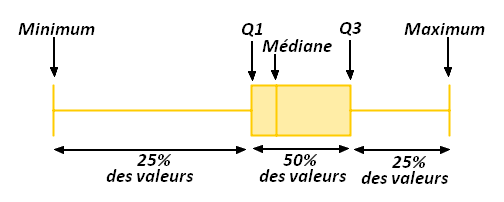
\includegraphics[width=0.6\textwidth]{BoxPlots.png}%
	\captionof{figure}{Composantes d'une boite à moustaches.}\label{labelname}%
\end{center}

\subsubsection{Variance et la Déviation standard}
La variance et la Déviation standard sont des mesures de dispersion des données.\\
Une faible dérivation standard indique que les données tendent à être proches de la moyenne, Tandis qu'une dérivation standard élevée implique le contraire.\\

La variance de N observations, $x_{1}, x_{2}, ... ,x_{N}$ ,d'un attribut numérique X est:
\begin{center}
	$\sigma^{2} = \frac{1}{N} * \sum_{i=1}^{N}{(x_{i}-\bar{x})^{2}} = (\frac{1}{N} * \sum_{i=1}^{N}{(x_{i})^{2}})-\bar{x}^{2}$
\end{center}
$\sigma$: est la dérivation standard.

\subsubsection{Représentations graphiques de descriptions statistiques ds données}

\textbf{Tracé de quartile}:Représente toutes les données, mettant en évidence aussi bien le comportement général que les valeurs inhabituelles.\\
\textbf{Tracé Q-Q}:Représente graphiquement les quantiles ($Q_{1},Q_{2},Q_{3}$) d'une distribution univariée par rapport aux quantiles d'une autre distribution.\\
\textbf{Histogrammes}:Représente la proportion de chaque catégorie. Lorsque les catégories ne sont pas de largeur uniforme l'on peut exploiter la surface des barres pour en tirer plus d'informations.En plus de s'adapter à tous type d'attribut.\\
\textbf{Nuages de points}:Permet un aperçu des données à deux variables, fait apparaitre les clusters et les outliers.

\section{Visualisation des données}
\subsection{Technique de visualisation Orientée pixels}
Chaque donnée de dimensions N, la visualisation se fera sur N fenêtres, une par dimension.Aussi les couleurs des pixels reflètent la valeur correspondante.

\subsection{Techniques de visualisation par projection géométrique}
Utilisée dans la compréhension de la distribution des données dans un espace multidimensionnel, citons quelques méthodes:\\
-Matrices de nuages de points.
-Nuages de points.
-Vues de la section
-Hyperslice
-Coordonnée parallèle
...etc

\subsection{Techniques de visualisation basées sur des icônes}
cette technique utilise de petites icônes pour représenter des images multidimensionnelles.
Citons deux méthodes des plus populaires: \textit{Chernoff Faces} et \textit{Stick Figures}.

\subsection{Techniques de visualisation hiérarchique}
Il s'agit d'un partitionnement hiérarchique en sous-espaces, parmi les méthodes connues:
"Worlds-within-Worlds","Tree-map", ...

\subsection{Visualiser des données complexes et des relations}
Permet de visualiser des données non numériques tel du texte (données complexe) et des réseaux sociaux (relations).
Comme un nuage de tags est une visualisation des statistiques des tags générés par l'utilisateur.


\section{Mesure de la similarité et de la disparité des données}
Mesure numérique du degré de ressemblance de deux objets, généralement ayant des valeurs entre o et 1.

\subsection{Matrice de données versus matrice de disparité}
\textbf{Matrice de données}: stockant les valeurs des données. sous la forme d'une table relationnelle (matrice) X objets x N attributs.\\

\textbf{ }
\textbf{matrice de disparité}: renferme la distance entre les objets d'un ligne et ceux d'une colonne. (matrice X Objets x X Objets).

\subsection{Mesures de proximité pour les attributs nominaux}
\textbf{Méthode 1:Simple correspondance:}
Matrice de disparité, avec:
\begin{center}
	$d(i,j) = \frac{p - m}{p} $
\end{center}
Avec : m: nombre de correspondance, p: nombre total de variables.\\
\textbf{Méthode 2: utiliser un grand nombre d'attributs binaires:}

\subsection{Mesures de proximité pour les attributs binaires}Il existe:\\
Mesure de distance pour les variables binaires symétriques.\\
Mesure de distance pour les variables binaires asymétriques\\
Coefficient de Jaccard (mesure de similarité pour les variables binaires asymétriques).\\

\subsection{Dissimilarité des données numériques: distance de Minkowski}
Cette mesure comprend la distance Euclidienne et la distance de Manhattan, sa formule : 
\begin{center}
	$d(i,j) = \sqrt[h]{|x_{i1}-x_{j1}|^h + |x_{i2}-x_{j2}|^h + ... + |x_{in}-x_{jn}|^h}$
\end{center}
Avec: n = nombre d'attributs, h = nombre réel tel que h $\geq$ 1.

\subsection{Mesures de proximité pour les attributs ordinaux}
les étapes suivantes sont nécessaires:\\
-Remplace $x_{if}$ par son rang.($r_{if} \in {1,...,M_{f}}$).\\
-Normalisez les variable sur [0, 1] en remplaçant le i-ème objet de la f-ème variable par:
\begin{center}
	$z_{if} = \frac{r_[if] - 1}{M_{if} - 1}$
\end{center}
-Mesurer la distance.

\subsection{Dissemblance des attributs de types mélangés}
Notre Dataset peut contenir tous les types d'attributs, calcule de la distance selon la formule:
\begin{center}
	$d(i,j) = \frac{\sum_{f=1}^{p}{\delta_{ij}^{(f)} d{ij}^{(f)}}}{\sum_{f=1}^{p}{\delta_{ij}^{(f)}}}$
\end{center}
Avec: f est binaire ou nominal,
$d{ij}^{(f)}$ = 0 si $x_{if}$ = $x_{jf}$ ou $d{ij}^{(f)}$ = 1 sinon
f est numérique: utilise la distance normalisée.
\subsection{Similitude cosinus}
C'est une mesure de la similarité qui peut être utilisée pour comparer des documents, de très grands nombres d'attributs, comme la fréquence des mot dans les documents (ou plusieurs mots peuvent avoir une fréquence = 0).\\
Soit x et y deux vecteurs de comparaison
\begin{center}
	$sim(x,y) = \frac{x\bullet y}{||x||*||y||}$
\end{center}
Avec: $||x||$ est la norme Euclidienne du vecteur $x = (x_{1}, x_{2}, ... , x_{n})$

\chapter{Pré-traitement des données[1]}
\vspace{-1 cm}

\section{Qualité des données : Pourquoi faire du prétraitement sur nos données ?}
On dira que les données sont de qualité si elles répondent aux exigences suivantes :\\
l'exactitude, exhaustivité, complétude,  cohérence, actualité (évolutif dans le temps), crédibilité et interprétabilité.\\
	
Mais avoir des données de qualité n'est pas chose facile , dans le monde réel beaucoup de facteurs rentrent en jeux pour compromettre  la qualité des données tel que :
\begin{itemize}
	\item  valeurs manquantes (donnée incomplète ) dans les tuples de données 
	\item  valeurs aberrantes (date de naissance 1700 par exemple "bruité") 
	\item inconsistance ou encore des valeurs dupliquées . 
	
\end{itemize} 

Si alors on plonge  directement dans l'exploration de nos données sans prêter attention à ces inconvenants là, la qualité des motifs ou modèles  sera affectés directement  ce qui causera un manque de crédibilité et de confiance dans ces derniers qui risquent être erronés.

\section{Data Cleaning}
L'une des principales approches de prétraitement des données , qui essaye de proposer des solutions aux différents problèmes citées plus .

\subsection{Valeurs manquantes}
Il existe diverse méthodes pour gérer les valeurs manquantes des données parmi elles :
\subsubsection{Ignorer le tuple}
cela consiste à renoncer à l'utilisation du tuple alors que ce dernier peut s'avérer intéressent par la suite, cette solution n'est efficace si la majorité de nos données souffrent d'un manque de valeurs d'un attribut ou deux .
\subsubsection{Remplir les valeurs manquantes manuellement}
Si la taille de nos données est conséquente cette méthode devient infaisable (elle prend énormément de temps) .
\subsubsection{Utilisation d'une valeur globale pour remplir les valeurs manquantes}
son inconvénient majeur est que lors de la fouille ou l'exploration ce genre de  valeurs globales peuvent être prise pour des concepts intéressent .
\subsubsection{Utilisation d'une mesure de la tendance centrale de l'attribut (par exemple, la moyenne ou la médiane)}
\subsubsection{Utilisez l'attribut moyenne ou médiane pour tous les échantillons appartenant à la même classe que le tuple donné }
\subsubsection{Utilisation de la valeur la plus probable}
ceci peut être fait grâce à la fonction de régression  , arbre de décision ou encore  l'algorithme naïf de bayes,c'est généralement la technique la plus utilisée  .


\subsection{Les données bruitées ou erronées ( Noisy data)}
Les données bruitées sont des données qui manquent d'incohérence comme des valeurs aberrantes ,plusieurs techniques ont été mise au point pour faire face à ce genre de problème ,on citera:
\subsubsection{Binning (nettoyer en enlevant des valeurs)}
Binning se repose principalement sur le trie des valeurs des données puis il effectuera un partitionnement uniforme  de façon à voir la même taille pour chaque partition ,ce qui permettra de consulter les voisins des valeurs erronées (une recherche locale) , le binning choisira par la suite de remplacer les valeurs aberrantes par la moyenne de la partition ou la médiane ou encore par le min si la valeur est plus proche du celui ci sinon par le max de l'intervalle de la  partition (le plus proche voisin).

\subsubsection{Régression}
Afin de remplacer les valeurs erronés on peut faire appelle à une fonction de régression linéaire 
qui inclut deux variables (attributs ) on donnera alors une valeur d'attribut pour prédire l'autre.
\begin{equation*}
	F(attribut_1)=attribut_2
\end{equation*}
ou bien une fonction de régression de dimension trois ou plus ou plusieurs attributs sont mise en jeux .
\begin{equation*}
	F(attribut_1,attribut_2,....,attribut_n)=attribut_j  \end{equation*}
\subsubsection{Analyse des outlier}
en utilisant le clustering 
\subsection{Data Cleaning comme un processus}
On peut résumer le nettoyage de données en des étapes élémentaires qui sont les suivantes:

\textbf{ Détection de divergence : }
\begin{itemize}
	\item Utilisez des métadonnées .
	\item Vérifiez la surcharge du champ.
	\item Vérifiez la règle d'unicité, la règle consécutive et la règle null.
	\item Utilisez des outils commerciaux.(data scrubbing (nettoyage) ,Data auditing( detecter des relations o corrélations)
	
\end{itemize}
\textbf{ Migration de données et intégration:}
\begin{itemize}
	\item Outils de migration de données
	\item Outils ETL (Extraction / Transformation / Loading)
\end{itemize}
\textbf{ Intégration des deux processus:}
Itératif et interactif 

\section{Intégration des données}
\subsection{Problème d'identification d'entité}
ce problème survient lorsque on à faire à des données collecter de plusieurs sources, l'identification d'entité consiste à retrouver des attributs  qui font référence à la même entité par exemple l'attribut id\_consommateur ou nb\_consommateur mais aussi la détection de différente structure d'un même attribut du diverse sources , généralement on utilise les méta données pour remédier à ce problème
\subsection{Analyse de redondance et de corrélation}
Lorsqu'un attribut peut être déduit à partir d'un autre attribut ou plus on dira qu'il est redondant, l'analyse de corrélation permet  de détecter la redondance  on citera :
\subsubsection{$X^2$ corrélation pour données nominales}
Pour les données nominales, une relation de corrélation entre deux attributs, A
et B , peut être découvert par un X2(  chi-carré) test,
Hypothèse : les deux distributions sont indépendantes
Les cellules (matrice r colonnes  c lignes) qui contribuent le plus à la valeur X2 sont celles dont le nombre réel (observé) est très différent du nombre attendu .
Plus la mesure X2 est grande, plus les variables sont susceptibles d'être liées.


\begin{equation*}
	X^2 = \sum_{i=1}^{C}\sum_{j=1}^{r}\frac{(o_{ij}- e_{ij})^2}{e_{ij}}
\end{equation*}
\begin{equation*}
	e_{ij}= \frac{count(A=a_{i})* count(B=b_{j})}{n}
\end{equation*}

c : valeurs distinctes que peut prendre l'attribut A

r :valeurs distinctes que peut prendre  l'attribut B

$o_{ij}$: fréquence observé de l'événement commun $A=a_{i},B=b_{j}$

$e_{ij}$: fréquence attendue (prévisible ) de l'événement commun $A=a_{i},B=b_{j}$

n: nombre de tuples totale

count($a_{i}$): nombre de tuple ayant la valeur $a_{i}$ pour A

count( $b_{j}$):nombre de tuple ayant la valeur $b_{j}$ pour B

\subsubsection{Coefficient de corrélation pour les données numériques} 
coefficient de corrélation de pearson :

\begin{equation*}
	r A,B= \frac{\sum_{i=1}^{n} (a_{i}-\bar{A})(b_{i}-\bar{B})}{n\sigma_{A} \sigma_{B} }= \frac{\sum_{i=1}^{n} (a_{i},b_{i})-n\bar{A}\bar{B}}{n\sigma_{A} \sigma_{B} }
\end{equation*}

$\bar{A}$:La moyenne des valeurs de l'attribut A.

$\bar{B}$:La moyenne des valeurs de l'attribut B.

$\sigma_{A}$: l'écart type de A

$\sigma_{B}$: l'écart type de B

$\sum_{i=1}^{n} (a_{i},b_{i})$: produit vectoriel


r A,B est une mesure entre -1 et 1 si la valeur est positive on dira que A ,B sont positivement corrélé  donc ils augmentent de façon proportionnelle, plus la valeur est proche de  1 plus ils sont corrélé , par contre si la valeur est négative on dira que A,B sont inversement proportionnelle .
à noter que si r A,B = 0 , A et B sont indépendants
\subsubsection{Covariance des données numériques}
Dans la théorie des probabilités et les statistiques, la corrélation et la covariance sont deux mesures similaires.

\begin{equation*}
	E(A)=\bar{A}=\frac{\sum_{i=1}^{n} a_{i}}{n}
\end{equation*}
\begin{equation*}
	E(B)=\bar{B}=\frac{\sum_{i=1}^{n} b_{i}}{n}
\end{equation*}
La covariance est défini comme :
\begin{equation*}
	Cov(A,B)=E((A-\bar{A})(B-\bar{B})) = \frac{\sum_{i=1}^{n} (a_{i}-\bar{A})(b_{i}-\bar{B})}{n }
\end{equation*}
\begin{equation*}
	r A,B= \frac{Cov(A,B)}{\sigma_{A}\sigma_{B}}
\end{equation*}
\begin{equation*}
	Cov(A,B)= E(A.B)-\bar{A}\bar{B}
\end{equation*}
Comme la corrélation numérique ,A,B sont dites indépendant alors leurs covariance est nulle , positivement proportionnelle si la covariance est positive et inversement proportionnelle si covariance est négative.
\subsection{Duplication de tuples}
c'est lorsqu'il y a deux ou plusieurs tuples identiques pour une donnée en cas de saisie de données unique.
\subsection{Détection et résolution de conflits de valeurs de données}

L’intégration de données implique également la
détection et résolution de conflits de valeurs de données
par exemple pour une même entité du monde réel, les valeurs d'attribut provenant de sources différentes peuvent varier.
Cela peut être dû à des différences de représentation, de mise à l'échelle ou d'encodage. Par exemple, un  poids (attribut) peut être stocké en unités métriques (kg) dans un système et impériale britannique  dans un autre (pound).

\section{Réduction de données}
Des techniques de réduction des données permettent d'obtenir une représentation réduite du Dataset, tout en maintenant l'intégrité du document d'origine.
Ainsi l'extraction de données devrait être plus efficace tout en produisant des résultats d'analyse quasi identiques.

\subsection{Les stratégies de réduction de données}
Les stratégies de réduction des données incluent:\\
 \textbf{La réduction de la dimensionnalité}: permet d'éliminer les attributs non pertinents et de réduire le bruit, parmi les techniques: les transformées en ondelettes et l'analyse en composantes principales.\\
 \textbf{La réduction de la numérotation}, elle remplacer le volume de données d'origine par une alternative, citons: les modèles de régression et log-linéaires, Histogrammes, regroupement, échantillonnage, Agrégation de cube de données.\\
 \textbf{La compression des données}:cette stratégie permet d'obtenir une représentation réduite ou $<<$compressée$>>$ des données d'origine.
 
 \subsection{Transformée en ondelettes}
C'est une technique de traitement du signal linéaire étroitement liée à la transformée de Fourier discrète qui, appliqué à un vecteur de données X, le transforme en un vecteur différent X' de
 coefficients d'ondelettes. En ne stockant qu'une petite fraction du plus fort des coefficients.
 
 \subsection{Analyse en composantes principales}
 Cette analyse permet de trouvez une projection qui englobe la plus grande quantité de variation dans les données.
 
 \subsection{Sélection de sous-attributs}
 Cette stratégie à fait ses preuves pour l'élimination d'attributs redondants et non pertinents.\\
 Quelques méthodes typiques de sélection d'attributs par heuristiques:
 Sélection pas à pas, élimination progressive, Combinaison de sélection en avant et d'élimination en arrière et Induction par arbre de décision.
 
\subsection{Modèles de régression et log-linéaires: Réduction de donnée paramétriques}
Des modèles de régression et log-linéaires fournissent une approximation des données fournies.\\
\textbf{Régression linéaire}: Données modélisées pour correspondre à une ligne droite.\\
\textbf{La régression linéaire multiple}:il s'agit d'une extension de la précédente, elle permet à une variable de réponse y, d'être modélisé comme une fonction linéaire de deux variables prédictives ou plus.\\
\textbf{Modèles log-linéaires}:Approximation des distributions de probabilité multidimensionnelles discrètes.

\subsection{Histogrammes}
Représente la distribution des données, Il divise les données en compartiments et garde la moyenne pour chacun d'eux.\\
Deux règles de partitionnement sont possibles: Largeur égale ou fréquence égale.\\
Utiles pour approximer les données éparses et denses, très asymétriques et uniformes.

\subsection{Clusterisation}
A pour but de partitionner les données en clusters en fonction de la similarité.

\subsection{Échantillonnage}
il permet à un grand ensemble de données d'être représenté par un échantillon de données aléatoire beaucoup plus petit.\\
Voici quelques type d'échantillonnage: Échantillonnage aléatoire simple, Échantillonnage sans remplacement, Échantillonnage avec remplacement, Échantillonnage stratifié.

\subsection{Agrégation de cube de données}
Il utilise le niveau le plus bas d'un cube de données (cuboïde de base), en utilisant la plus petite représentation qui soit suffisante pour résoudre la tâche.


\section{Transformation et discrétisation des données}
\subsection{Vue d'ensemble des stratégies de transformation de données}
\textbf{Lissage}: Il permet d'éliminer le bruit des données. Les techniques incluent le binning,
régression et clustering.\\
\textbf{Construction d'attribut}:de nouveaux attributs sont ajoutés à partir de l'ensemble d'attributs donné pour aider le processus d'exploration.\\
\textbf{Agrégation}:opération de résumé ou fonction d'agrégation, généralement utilisée dans la construction du cube de données.\\
\textbf{Normalisation}:mises à l'échelle des valeurs des attributs de manière à réduire la plage de données.\\
\textbf{Discrétisation}: lorsque les valeurs brutes d'un attribut numérique sont remplacées par étiquettes d'intervalle.\\
\textbf{Génération de hiérarchie de concepts pour les données nominales}:pour des attributs qui peuvent être généralisé.

\subsection{Transformation de données par normalisation}
La normalisation des données tente d'attribuer un poids égal à tous les attributs, pour n'en favoriser aucun. Il existe de nombreuses méthodes de normalisation des données. Nous étudierons la normalisation min-max, z-score et par mise à l'échelle décimale. Pour ce qui suit, Soit A un attribut numérique avec n valeurs observées, $v_{1},v_{2}, ... , v_{n}$.\\
\textbf{normalisation min-max}:effectue une transformation linéaire sur les données d'origine.\\
la normalisation d'un $v_{i}$ de [$min_{A},max_{A}$] dans [$new\_min_{A},new\_max_{A}$]
\begin{center}
	$v_{i}' = \frac{v_{i} - min_{A}}{max_{A} - min_{A}} * (new\_max_{A} - new\_min_{A}) + new\_min_{A}$
\end{center}
\textbf{normalisation z-score}:les valeurs pour un attribut A, sont normalisés en fonction de la moyenne et l'écart type.
\begin{center}
		$v_{i}' = \frac{v_{i} - \bar{A}}{\sigma_{A}}$
\end{center}
\textbf{normalisation par mise à l'échelle décimale}:normalise en déplaçant le point décimal des valeurs d'attribut A. (j est le plus petit entier tel que $max(|v_{i}|) <1$)
\begin{center}
	$v_{i}' = \frac{v_{i}}{10^{j}}$
\end{center}

\subsection{Discrétisation par binning}
Le binning est une technique de fractionnement par le haut.

\subsection{Discrétisation par analyse d'histogramme}
Un histogramme partitionne les valeurs d'un attribut A, en plages disjointes appelées compartiments.

\subsection{Discrétisation par cluster, arbre de décision,et analyses de corrélation}
Il s'agit dans l'ordre de :"fusion non supervisée, scission ascendante ou ascendante","scission supervisée et descendante" et "fusion non supervisée et non supervisée".

\subsection{Génération de hiérarchie de concepts pour les données nominales}
Organise les valeurs d'attributs de manière hiérarchique et est généralement associé à chaque dimension d'un entrepôt de données.citons 4 méthodes:\\
\textbf{ }\\
	- Spécification d'un classement partiel des attributs explicitement au niveau du schéma par	utilisateurs ou experts.\\
	- Spécification d'une partie d'une hiérarchie par regroupement explicite de données.\\
	- Spécification de seulement un ensemble partiel d'attribut.\\
	- Génération automatique de hiérarchies par l'analyse du nombre de valeurs distinctes.


\chapter*{Bibliographie}

 \textbf{[1]}Jiawei Han, Micheline Kamber, Jian Pei."Data-Mining Concepts and Techniques", 3rd Edition Morgan Kaufmann (2011).\\
\end{document}